Image generation has long been at the forefront of research in computer vision and artificial intelligence. From the initial forays with Variational Autoencoders (VAEs) \cite{Kingma2013} and Generative Adversarial Networks (GANs) \cite{Goodfellow2014} to the recent breakthroughs in photorealistic image synthesis, the field has seen rapid evolution. VAEs, which are neural networks designed to encode and decode images, laid the groundwork for understanding complex data distributions. GANs, comprising two competing networks, further advanced the capability to generate new, high-quality images by learning to mimic the distribution of real images.

Diffusion models have disrupte the longstanding dominance of GANs \cite{Goodfellow2014} and VAEs \cite{Kingma2013} in the realm of image generation. These novel generative models are currently receiving significant attention. Originating from the domain of thermodynamics, the concept of diffusion models introduces a fresh approach to image generation \cite{Sohl-Dickstein2015}. The underlying idea posits that gradually introducing noise into an image until it is completely transformed into noise—and then reversing this process—mirrors the core principles of generating images. This reversal process, if successfully learned by deep learning techniques, could revolutionize image generation. Further, the mathematical foundation of diffusion models was solidified with the use of Markov chains in Denoising Diffusion Probabilistic Models (DDPM) \cite{DDPM}, providing a robust theoretical framework that enhances our understanding and capabilities in generating complex images.

The advent of open-source initiatives like Stability.ai's Stable Diffusion marked a significant leap forward. These models have democratized access to advanced image generation technologies, catalyzing both academic research and product innovation. Unlike their predecessors, diffusion models generate images through a process of gradually refining random noise, aligning more closely with how humans might imagine and create images from scratch \cite{LDM}.

Recently, these models have been enhanced by training on image-caption pairs, leveraging techniques such as those introduced by CLIP (Contrastive Language–Image Pre-training) to align images with text prompts more effectively \cite{CLIP}. To navigate away from the adversarial nature of GANs, Classifier-Free Guidance (CFG) emerged as a method to improve the fidelity and diversity of generated images without the need for a discriminator network \cite{CFG}.

Despite these advancements, the quest for models that can faithfully adhere to all elements of a text prompt remains ongoing. The gap between the complexity of human language and the interpretative capability of AI models poses a significant challenge. Innovations like ControlNet offer a promising direction by incorporating additional inputs such as depth maps and pose maps to provide nuanced control over the image generation process \cite{ControlNet}. However, achieving perfect alignment between text prompts and generated images is still a complex challenge that the field continues to grapple with.

Moreover, these image generation models still struggle with finer details, such as accurately generating text within images or getting the right number of fingers on a hand. These seemingly minor inaccuracies highlight the ongoing challenges in creating truly lifelike and accurate images.

The application of diffusion models extends beyond mere image creation; they have been successfully applied to image editing, video generation and editing, 3D model generation from text or images, and even document layout generation. This survey paper aims to delve into the multifaceted world of diffusion models, exploring their components, evolutionary trajectory, limitations, and the ingenious solutions devised to overcome these hurdles.

A comprehensive mindmap detailing the development and evolution of diffusion models is included in Figure 1. This visual representation provides an overview of the key milestones, technologies, and innovations that have shaped the current landscape of diffusion models.

As we chart the course of diffusion models from their inception to their current state, and look towards the future, it becomes evident that while significant strides have been made, the journey is far from over. The potential for further breakthroughs and applications is vast, promising a dynamic and exciting future for image generation technology.


\begin{figure}[]
    \centering
    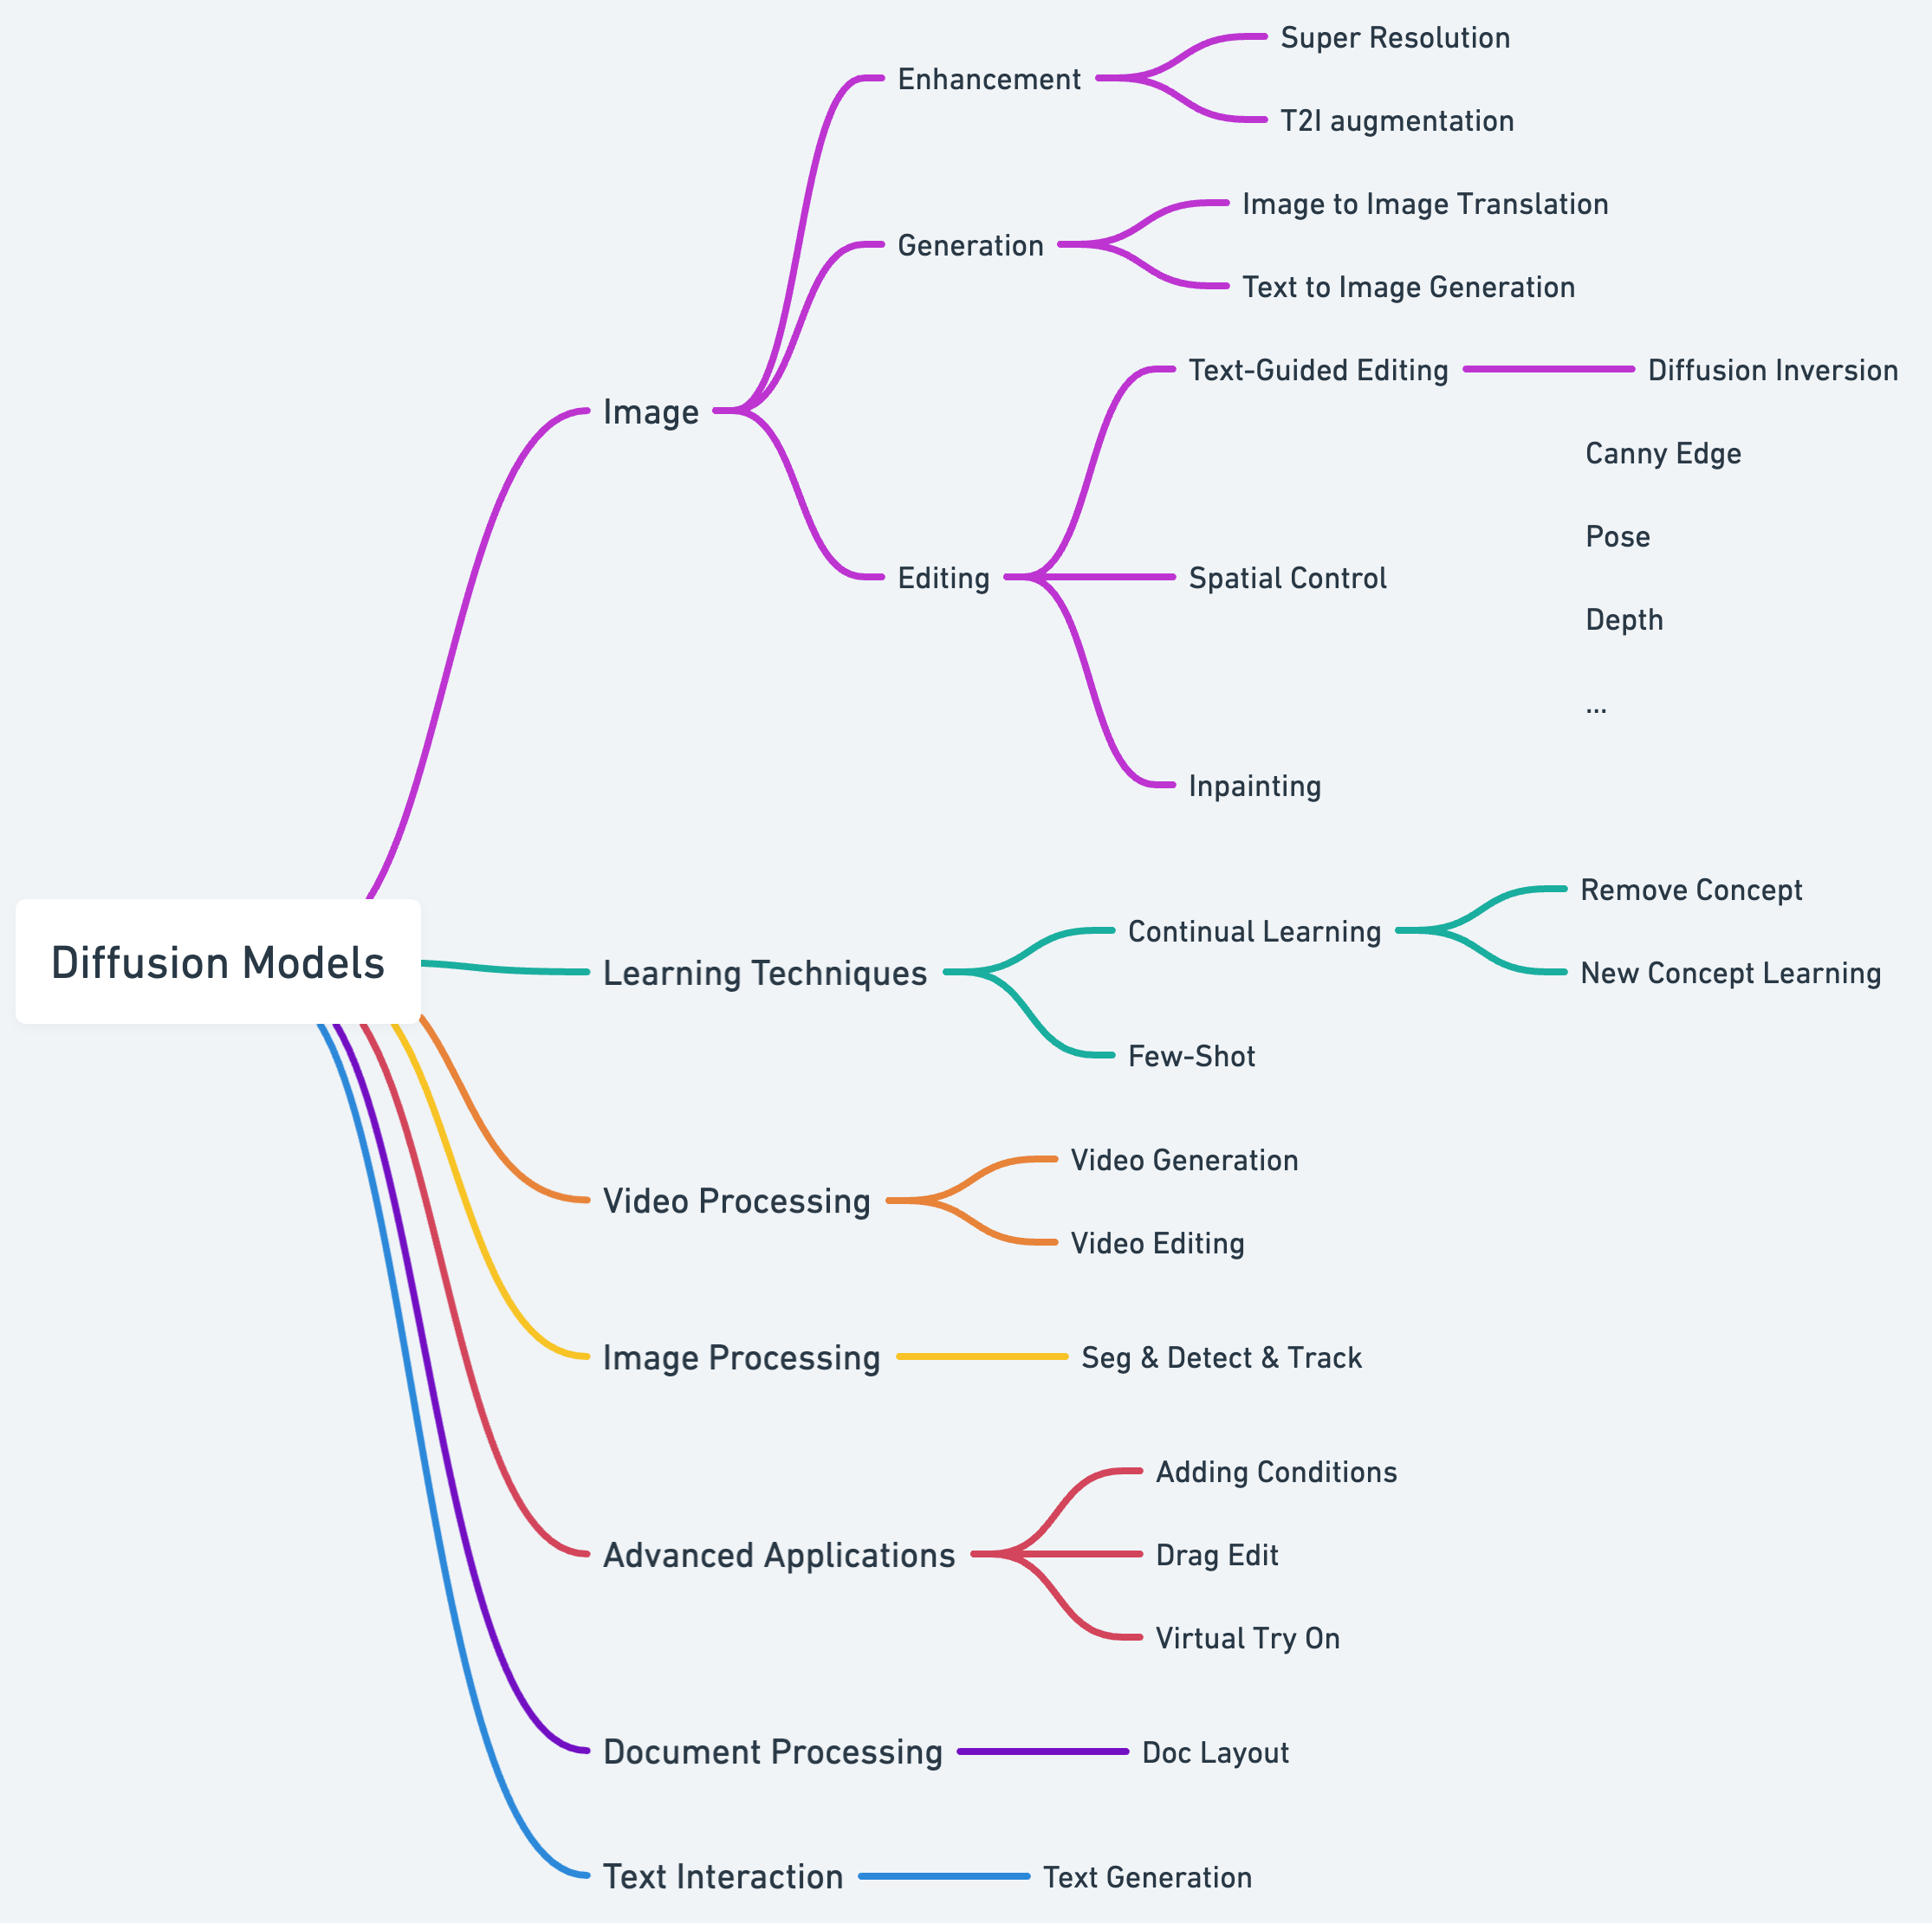
\includegraphics[width=\textwidth]{images/mind-map.png}
    \caption{Mind Map of diffusion models}
    \end{figure}